\documentclass[tikz]{standalone}
\usetikzlibrary{angles, quotes, calc, arrows.meta}

\begin{document}
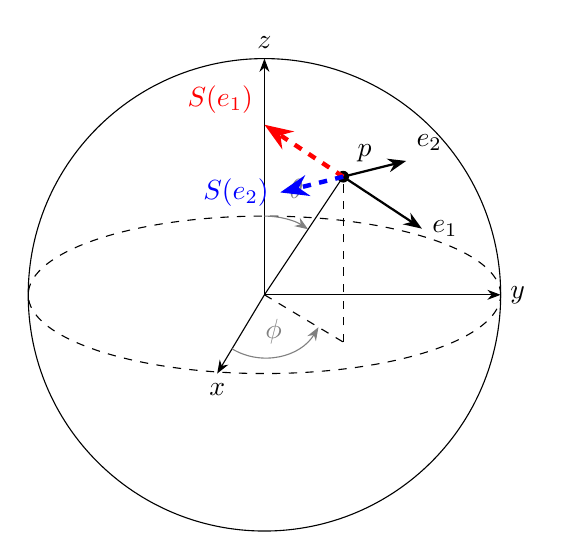
\begin{tikzpicture}[>=Stealth]
	% --- 1. SETUP (Matching your snippet) ---
	\def\r{3}
	\coordinate (O) at (0, 0);
	
	% Define Axes Tips
	\coordinate (x1) at (-\r/5, -\r/3);
	\coordinate (x2) at (\r, 0);
	\coordinate (x3) at (0, \r);
	
	% Define Point p (a) and Projection (phi) using your exact coords
	\coordinate (p) at (\r/3, \r/2);      
	\coordinate (proj) at (\r/3, -\r/5);  
	
	% --- 2. DRAW SPHERE & AXES ---
	\draw (O) circle (\r);
	\draw[dashed] (O) ellipse (\r{} and \r/3);
	
	\draw[->] (O) -- (x1) node[below] {$x$};
	\draw[->] (O) -- (x2) node[right] {$y$};
	\draw[->] (O) -- (x3) node[above] {$z$};
	
	% Radius Line (needed for Theta to sit on)
	\draw (O) -- (p);
	
	% Projection Lines
	\draw[dashed] (O) -- (proj);
	\draw[dashed] (proj) -- (p);
	
	
	% --- 3. ANGLES (The Fix) ---
	
	% Theta: From p UP to x3 (Counter-clockwise logic)
	% This ensures the small interior angle is drawn.
	\pic [draw=gray, text=gray, <-, "$\theta$", angle eccentricity=1.4, angle radius=1cm] {angle = p--O--x3};
	
	% Phi: From x1 to Projection
	\pic [draw=gray, text=gray, ->, "$\phi$", angle radius=0.8cm] {angle = x1--O--proj};
	
	
	% --- 4. TANGENT BASIS VECTORS ---
	
	% e1 (South): Tangent to meridian
	% Visually perpendicular to the radius O->p, pointing down.
	% Radius is approx (1, 1.5). Perpendicular is (1.5, -1). 
	% We scale it to be a reasonable size vector.
	\coordinate (e1_vec) at (1.0, -0.66); 
	
	% e2 (East): Tangent to parallel
	% Visually horizontal, slightly perspective-tilted.
	\coordinate (e2_vec) at (0.8, 0.2); 
	
	% --- 5. DRAW VECTORS ---
	
	% Point p
	\node[circle, fill, inner sep=1.5pt, label={above right:$p$}] at (p) {};
	
	% Basis Vectors (Solid Black)
	\draw[thick, ->] (p) -- ++(e1_vec) node[right] {$e_1$};
	\draw[thick, ->] (p) -- ++(e2_vec) node[above right] {$e_2$};
	
	% Shape Operator Vectors (Dashed Colored)
	% S(e) = -e (Exact opposite)
	\draw[red, ultra thick, dashed, ->] (p) -- ++($-1*(e1_vec)$) node[above left] {$S(e_1)$};
	\draw[blue, ultra thick, dashed, ->] (p) -- ++($-1*(e2_vec)$) node[left] {$S(e_2)$};
	
\end{tikzpicture}
\end{document}